\subsection{ソフトウェアアーキテクチャ過程}

\subsubsection*{アーキテクチャ過程の全体像}
\addcontentsline{toc}{subsubsection}{アーキテクチャ過程の全体像}
アーキテクチャ設計は、単純な一方向の工程ではない。一般的には、関心事と要求を理解する分析、候補解を作る統合、候補解を検証する評価を反復する。要求が変わり、制約が明らかになり、評価で問題が見つかるたびに、分析と統合に戻る。

\subsubsection{文脈の中のアーキテクチャ}
アーキテクチャは真空中で作られるものではない。どの開発ライフサイクルを使うか、製品系列の中にあるか、企業全体のアーキテクチャに従うか、システム・オブ・システムズの一部かによって、作り方が変わる。

伝統的なライフサイクルでは、要求に基づいてアーキテクチャ設計段階を置くことが多い。このとき、すべての要求が同じ重要度を持つわけではない。アーキテクチャに強く影響する要求、すなわち ASR を見極める必要がある。

製品系列や製品ファミリでは、共通のアーキテクチャが先に作られ、それを土台として個別製品が作られる。個別製品は、共通部分と可変部分を持つ。共通アーキテクチャは再利用性を高めるが、過度に固定すると個別製品の自由度を下げる。

アジャイル開発では、明示的なアーキテクチャ設計段階が小さいことがあり、コードからアーキテクチャが「創発する」と説明されることもある。この考え方は、利用者中心の情報システムではうまく働く場合がある。しかし、組込みシステム、サイバーフィジカルシステム、安全性が重要なシステムでは、利用者物語に現れにくい重要品質があるため、意識的なアーキテクチャ検討が必要である。

企業アーキテクチャやシステム・オブ・システムズの文脈では、上位のアーキテクチャが個別ソフトウェアの要求や制約になる。仕様、API、準拠試験、標準インタフェースなどを通じて制約が課される。

\paragraph{アーキテクチャと設計の関係}
アーキテクチャと設計の境界は、しばしば曖昧である。アーキテクチャはソフトウェア設計から発展してきた分野であり、設計の一部として扱われることもある。しかし、実務上は区別して考えると理解しやすい。

\par\smallskip\noindent\refstepcounter{table}\label{tab:ch02-05}\textbf{表 \thetable: 第02章 ソフトウェアアーキテクチャ 表05}\par\smallskip
\begin{longtable}{P{0.22\linewidth}P{0.38\linewidth}P{0.32\linewidth}}
\toprule
観点 & アーキテクチャ & 設計 \\
\midrule
扱う範囲 & システム全体、環境、主要構成、品質特性、進化原則である。 & 構成要素の詳細、データ構造、アルゴリズム、実装方法である。 \\
要求との関係 & 要求を受けるだけでなく、利害関係者との交渉を通じて要求を形作ることがある。 & 既に定義された要求とアーキテクチャ制約を満たす方法を具体化する。 \\
変更影響 & 後から変更すると広範囲に影響しやすい。 & 比較的局所的に変更できる場合が多い。 \\
主な成果物 & アーキテクチャ記述、ビュー、意思決定記録、原則である。 & 詳細設計、インタフェース仕様、クラス設計、アルゴリズム設計である。 \\
\bottomrule
\end{longtable}

\begin{statementbox}{見分け方}
「この判断を後から変えると、多くの構成要素、品質特性、組織分担、運用方法に影響するか」と問う。影響が広ければ、アーキテクチャ判断である可能性が高い。
\end{statementbox}

\subsubsection{アーキテクチャ設計}
アーキテクチャ設計とは、設計原則と方法を使い、ソフトウェアアーキテクチャを作成し、記録する活動である。ここでは、システムの主要構成要素、その責任、性質、インタフェース、相互作用、環境との関係を決める。

典型的な関心事には、次のものがある。
\begin{itemize}
  \item 全体のアーキテクチャ様式と計算パラダイムである。
  \item システムを主要構成要素へ分割する方法である。
  \item 構成要素間の通信、同期、データ交換、制御の流れである。
  \item 関心事と設計責任をどの構成要素に割り当てるかである。
  \item 構成要素のインタフェースである。
  \item 性能、拡張性、資源消費、信頼性への対応である。
  \item 安全性やセキュリティのような全体横断的関心事への対応である。
\end{itemize}

アーキテクチャ設計は、\keyterm{分析}、\keyterm{統合}、\keyterm{評価}の三つの活動を反復する。

\paragraph{アーキテクチャ分析}
アーキテクチャ分析は、アーキテクチャ上重要な要求、すなわち ASR を集め、整理する活動である。ASR は、アーキテクチャに影響する要求である。たとえば、厳しい応答時間、大量アクセスへの拡張性、高い可用性、法規制への適合、強いセキュリティ、外部システムとの接続方式などが該当する。

分析では、既知の要求、利害関係者のニーズ、環境制約、上位アーキテクチャ、利用可能な資源を確認する。要求と制約の組合せが実現困難な場合には、利害関係者と交渉し、期待や要求を調整する必要がある。

\paragraph{アーキテクチャ統合}
アーキテクチャ統合は、分析で見つかった問題に対して候補解を作る活動である。構成要素をどう分けるか、どの様式を採るか、どの技術を使うか、どの品質特性をどの戦術で満たすかを検討する。

ここで重要なのは、局所的に最適な解が全体として最適とは限らないことである。性能を高める候補解が変更容易性を下げることがある。セキュリティを高める候補解が使いやすさを下げることがある。統合は、複数の関心事の相互作用を考慮する活動である。

\paragraph{アーキテクチャ評価}
アーキテクチャ評価は、選んだ候補解が ASR を満たすかを確認し、手戻りが必要な箇所を見つける活動である。評価は最後に一度だけ行うものではない。分析と統合の途中で繰り返し行い、問題を早く見つけるほど、修正費用を抑えられる。

\begin{figure}[htbp]
\centering
\IfFileExists{assets/generated_figures/ch02/fig-ch02-07.png}{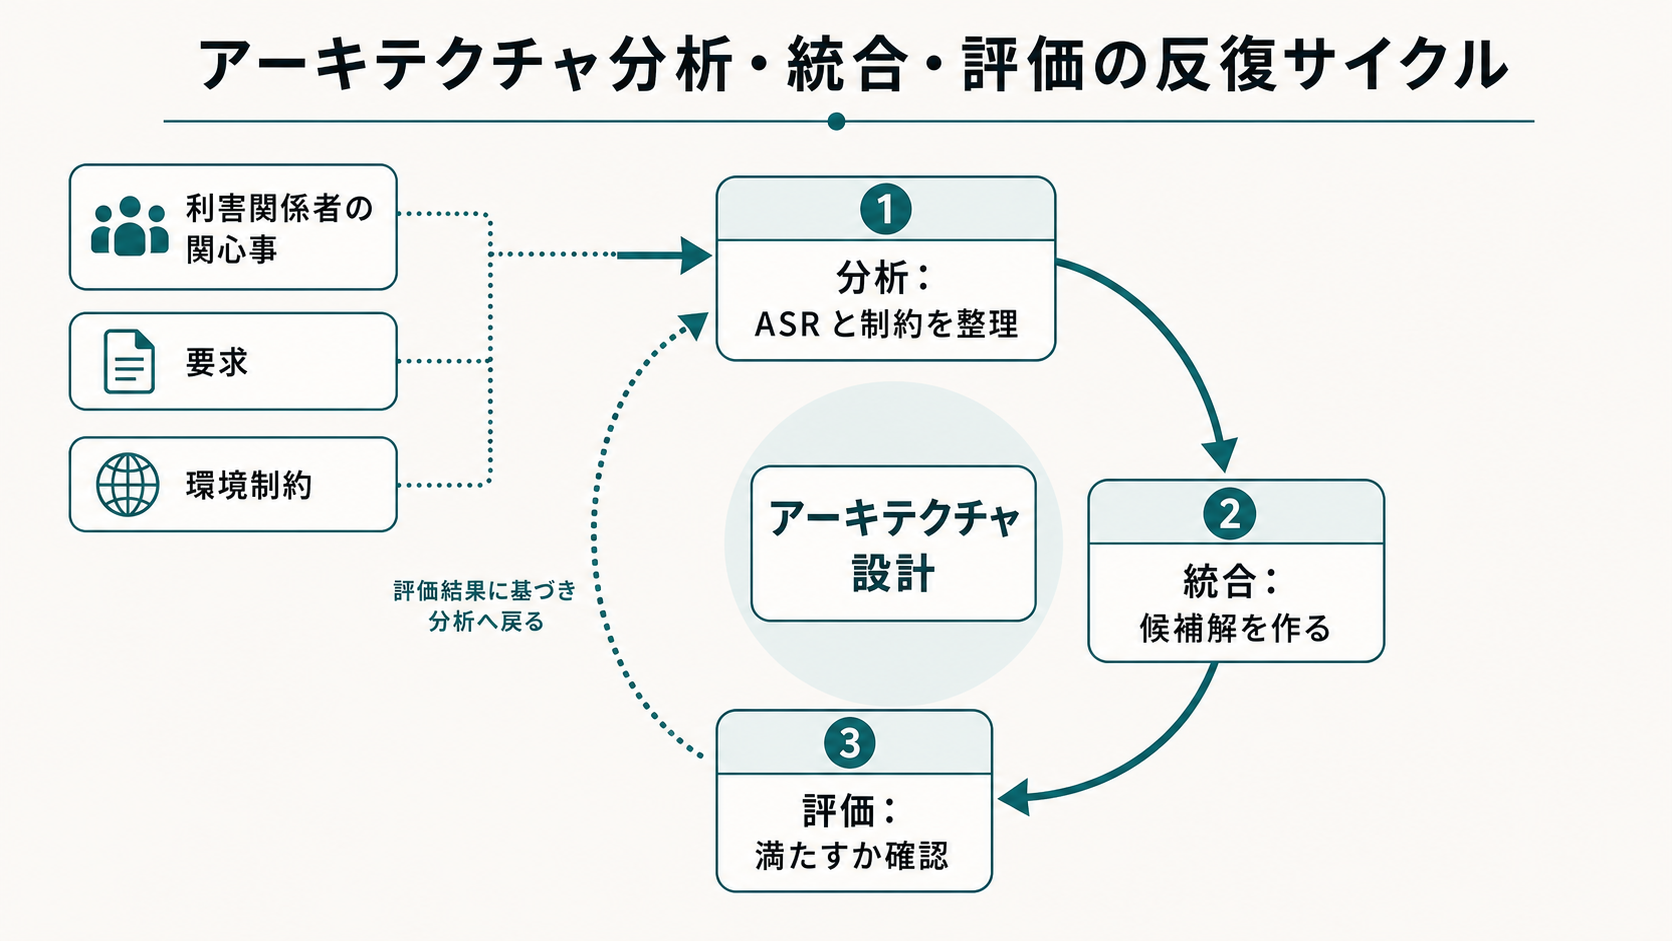
\includegraphics[width=0.96\linewidth]{assets/generated_figures/ch02/fig-ch02-07.png}}{\fbox{\parbox[c][48mm][c]{0.9\linewidth}{\centering 画像生成待ち\\アーキテクチャ分析・統合・評価の反復サイクル}}}
\caption{アーキテクチャ分析・統合・評価の反復サイクル}
\label{fig:ch02-07}
\end{figure}

\subsubsection{アーキテクチャの実践、方法、戦術}
アーキテクチャの実践には、多くの方法がある。方法とは、関心事の発見、要求整理、候補解作成、文書化、レビュー、評価をどの順序で行うかを定める作業手順である。戦術とは、特定の品質特性を満たすための小さな設計上の手段である。

たとえば、可用性を高めるには冗長化、監視、障害切替が使われることがある。性能を高めるにはキャッシュ、非同期処理、並列化が使われることがある。変更容易性を高めるには抽象化、疎結合、情報隠蔽が使われることがある。セキュリティを高めるには認証、認可、入力検証、監査ログが使われることがある。

\begin{statementbox}{注意}
戦術は魔法の解決策ではない。どの戦術にも副作用がある。キャッシュは性能を高めるが、整合性管理を難しくすることがある。冗長化は可用性を高めるが、費用と運用複雑性を増やすことがある。
\end{statementbox}

\subsubsection{大規模なアーキテクチャ活動}
アーキテクチャ設計は、ライフサイクル上の一段階を指すことがある。しかし、広い意味のアーキテクティングは、それだけではない。大規模な組織やシステムでは、個別システムのアーキテクチャが、企業アーキテクチャ、製品系列アーキテクチャ、システム・オブ・システムズのアーキテクチャと関係する。

このような文脈では、次の活動が重要になる。
\begin{itemize}
  \item \keyterm{アーキテクチャ実装管理}：実装がアーキテクチャに従っているかを確認する。
  \item \keyterm{アーキテクチャ保守}：実装後もアーキテクチャを管理し、拡張する。
  \item \keyterm{アーキテクチャ管理}：組織内の複数アーキテクチャの関係を管理する。
  \item \keyterm{アーキテクチャ知識管理}：意思決定、教訓、仕様、文書などを再利用可能な資産として残す。
\end{itemize}

大規模なアーキテクチャ活動では、個別システムの最適化だけでは不十分である。組織全体で一貫性、相互運用性、再利用性、進化可能性を保つ必要がある。
